\documentclass{article}
\usepackage{tikz}
\usetikzlibrary{positioning,calc,shapes.geometric}
\makeatletter
% Print an anchor in cm (1cm = 28.45274pt) for the scene oracle.
\newcommand\refanchor[2]{%
  \pgfpointanchor{#1}{#2}%
  \pgfmathsetmacro\refx{\pgf@x/28.45274}%
  \pgfmathsetmacro\refy{\pgf@y/28.45274}%
  \typeout{REF #1.#2 \refx\space\refy}}
\makeatother
\begin{document}

\begin{tikzpicture}[every node/.style={inner sep=0pt, outer sep=0pt}]
  \node (a) at (0,0) {\rule{1cm}{5mm}};
  \node (b) [right=of a] {\rule{1cm}{5mm}};
  \node (c) [below=2cm of a] {\rule{1cm}{5mm}};
  \node (d) [above right=of b] {\rule{1cm}{5mm}};
  \node (e) [below left=1cm and 2cm of a] {\rule{1cm}{5mm}};
  \node (f) [on grid, right=of a] {\rule{1cm}{5mm}};
  \node (g) [above right=1cm of b] {\rule{1cm}{5mm}};
  \node (h) [circle, right=5mm of b] {\rule{1cm}{5mm}};
  \node (k) [right=of a, on grid] {\rule{1cm}{5mm}};
  \node (n) [above=3mm] at (0,4) {\rule{1cm}{5mm}};
  \coordinate (m1) at ($(a)!0.5!(b)$);
  \coordinate (m2) at ($(a)+(1,2)$);
  \coordinate (m3) at ($(a)!1cm!(c)$);
  \coordinate (m4) at ($(a)!0.5!90:(b)$);
  \coordinate (m5) at ($(a)!(d)!(b)$);
  \coordinate (m6) at ($2*(b)-(a)$);
  \coordinate (m7) at ($(a.north east)+(0.5,0)$);
  \coordinate (m8) at ($(a)!0.25!(b)!0.5!(c)$);
  \coordinate (m9) at ($(a)!0.5!($(b)+(0,2)$)$);
  \refanchor{a}{center}
  \refanchor{b}{center}
  \refanchor{c}{center}
  \refanchor{d}{center}
  \refanchor{e}{center}
  \refanchor{f}{center}
  \refanchor{g}{center}
  \refanchor{h}{center}
  \refanchor{k}{center}
  \refanchor{n}{center}
  \refanchor{m1}{center}
  \refanchor{m2}{center}
  \refanchor{m3}{center}
  \refanchor{m4}{center}
  \refanchor{m5}{center}
  \refanchor{m6}{center}
  \refanchor{m7}{center}
  \refanchor{m8}{center}
  \refanchor{m9}{center}
\end{tikzpicture}

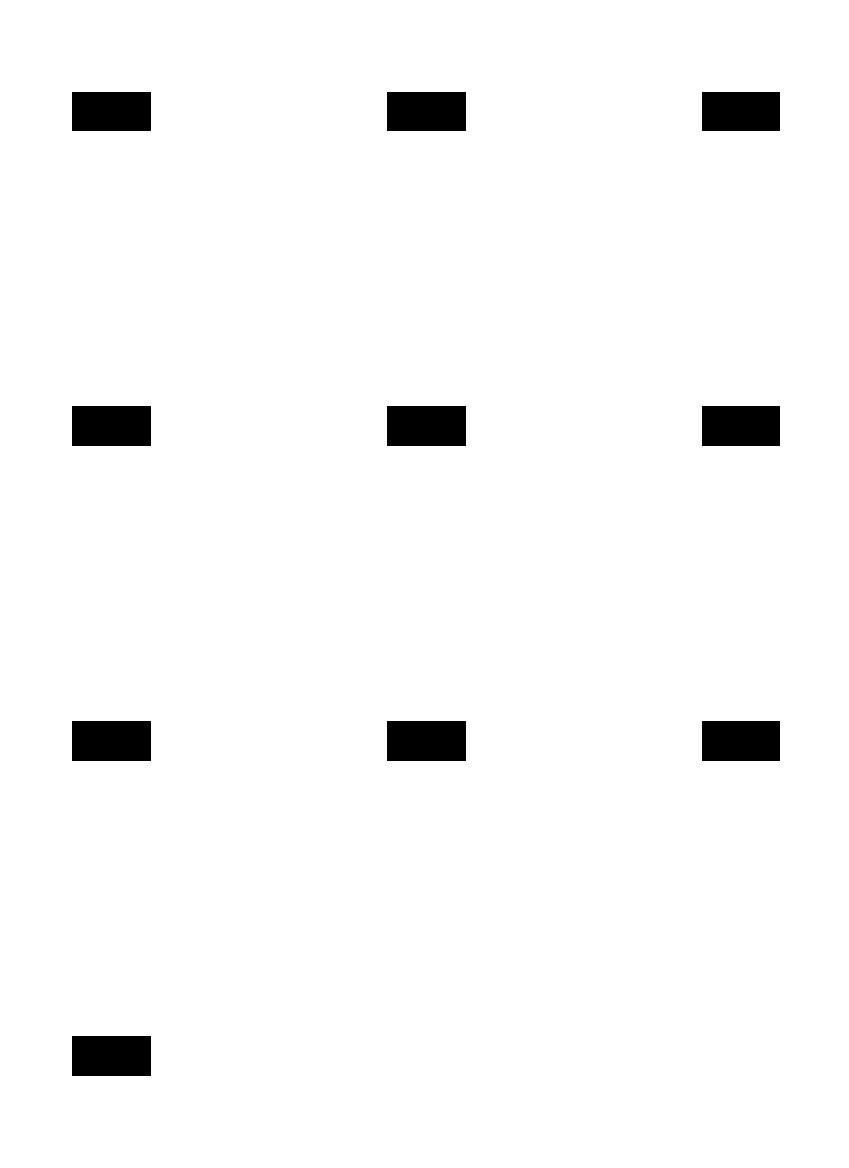
\begin{tikzpicture}[every node/.style={inner sep=0pt, outer sep=0pt}]
  \node[regular polygon, regular polygon sides=6] (r) at (0,0) {\rule{1cm}{5mm}};
  \node[regular polygon] (p) at (4,0) {\rule{1cm}{5mm}};
  \node[star, star points=5] (s) at (8,0) {\rule{1cm}{5mm}};
  \node[ellipse] (el) at (0,-4) {\rule{1cm}{5mm}};
  \node[diamond] (dm) at (4,-4) {\rule{1cm}{5mm}};
  \node[diamond, aspect=2] (da) at (8,-4) {\rule{1cm}{5mm}};
  \node[trapezium] (t) at (0,-8) {\rule{1cm}{5mm}};
  \node[trapezium, trapezium left angle=120, trapezium right angle=70] (t2) at (4,-8) {\rule{1cm}{5mm}};
  \node[circle] (ci) at (8,-8) {\rule{1cm}{5mm}};
  \node[regular polygon, regular polygon sides=4, minimum size=3cm] (q) at (0,-12) {\rule{1cm}{5mm}};
  \refanchor{r}{north}
  \refanchor{r}{east}
  \refanchor{r}{30}
  \refanchor{p}{north}
  \refanchor{p}{south}
  \refanchor{p}{east}
  \refanchor{s}{north}
  \refanchor{s}{south}
  \refanchor{s}{east}
  \refanchor{el}{north}
  \refanchor{el}{east}
  \refanchor{el}{north east}
  \refanchor{dm}{north}
  \refanchor{dm}{east}
  \refanchor{dm}{north east}
  \refanchor{da}{north}
  \refanchor{da}{east}
  \refanchor{t}{north}
  \refanchor{t}{south}
  \refanchor{t}{east}
  \refanchor{t}{south west}
  \refanchor{t}{north west}
  \refanchor{t2}{south west}
  \refanchor{t2}{north west}
  \refanchor{t2}{south east}
  \refanchor{t2}{north east}
  \refanchor{ci}{east}
  \refanchor{ci}{north east}
  \refanchor{q}{north}
  \refanchor{q}{east}
\end{tikzpicture}
\end{document}
